\section{Tips and Tricks}

Practitioners use several tricks to improve the performance of GANs.
It can be difficult to tell how effective some of these tricks are;
many of them seem to help in some contexts and hurt in others.
These should be regarded as techniques that are worth trying out,
not as ironclad best practices.

NIPS 2016 also featured a workshop on adversarial training, with
an invited talk by Soumith Chintala called "How to train a GAN."
This talk has more or less the same goal as this portion of the tutorial,
with a different collection of advice.
To learn about tips and tricks not included in this tutorial, check
out the GitHub repository associated with Soumith's talk:

\url{https://github.com/soumith/ganhacks}


\subsection{Train with labels}

Using labels in any way, shape or form almost always results in a dramatic
improvement in the subjective quality of the samples generated by the model.
This was first observed by \citet{denton2015deep}, who built class-conditional
GANs that generated much better samples than GANs that were free to generate
from any class.
Later, \citet{Salimans-et-al-arxiv2014} found that sample quality improved
even if the generator did not explicitly incorporate class information; training
 the discriminator to recognize specific classes of real objects is sufficient.

 It is not entirely clear why this trick works.
 It may be that the incorporation of class information gives the training
 process useful clues that help with optimization.
 It may also be that this trick gives no objective improvement in sample quality,
 but instead biases the samples toward taking on properties that the human
 visual system focuses on.
 If the latter is the case, then this trick may not result in a better model
 of the true data-generating distribution, but it still helps to create media
 for a human audience to enjoy and may help an RL agent to carry out tasks
 that rely on knowledge of the same aspects of the environment that are relevant
 to human beings.

 It is important to compare results obtained using this trick only to other
 results using the same trick; models trained with labels should be compared
 only to other models trained with labels, class-conditional models should
 be compared only to other class-conditional models.
 Comparing a model that uses labels to one that does not is unfair and an
 uninteresting benchmark, much as a convolutional model can usually be expected
 to outperform a non-convolutional model on image tasks.

\subsection{One-sided label smoothing}
\label{sec:label_smooth}

GANs are intended to work when the discriminator estimates a ratio of two
densities, but deep neural nets are prone to producing highly confident
outputs that identify the correct class but with too extreme of a probability.
This is especially the case when the input to the deep network is adversarially
constructed; the classifier tends to linearly extrapolate and produce
extremely confident predictions \citep{Goodfellow-2015-adversarial}.

To encourage the discriminator to estimate soft probabilities rather than
to extrapolate to extremely confident classification, we can use a technique
called \newterm{one-sided label smoothing} \citep{Salimans-et-al-arxiv2014}.

Usually we train the discriminator using \eqref{eq:discriminator_cost}.
We can write this in TensorFlow \citep{tensorflow} code as:
\begin{lstlisting}
d_on_data = discriminator_logits(data_minibatch)
d_on_samples = discriminator_logits(samples_minibatch)
loss = tf.nn.sigmoid_cross_entropy_with_logits(d_on_data, 1.) + \
       tf.nn.sigmoid_cross_entropy_with_logits(d_on_samples, 0.)
\end{lstlisting}

The idea of one-sided label smoothing is to replace the target for the real examples
with a value slightly less than one, such as .9:

\begin{lstlisting}
loss = tf.nn.sigmoid_cross_entropy_with_logits(d_on_data, .9) + \
       tf.nn.sigmoid_cross_entropy_with_logits(d_on_samples, 0.)
\end{lstlisting}

This prevents extreme extrapolation behavior in the discriminator; if it learns
to predict extremely large logits corresponding to a probability approaching $1$
for some input, it will be penalized and encouraged to bring the logits back
down to a smaller value.

It is important to not smooth the labels for the fake samples.
Suppose we use a target of $1-\alpha$ for the real data and a target of $0+\beta$
for the fake samples.
Then the optimal discriminator function is
\[ D^*(\vx) = \frac{(1-\alpha) \pdata(\vx) + \beta \pmodel(\vx)} { \pdata(\vx) + \pmodel(\vx) }.\]

When $\beta$ is zero, then smoothing by $\alpha$ does nothing but scale down the optimal value
of the discriminator.
When $\beta$ is nonzero, the shape of the optimal discriminator function changes.
In particular, in a region where $\pdata(\vx)$ is very small and $\pmodel(\vx)$ is larger,
$D^*(\vx)$ will have a peak near the spurious mode of $\pmodel(\vx)$.
The discriminator will thus reinforce incorrect behavior in the generator; the generator
will be trained either to produce samples that resemble the data or to produce samples
that resemble the samples it already makes.

One-sided label smoothing is a simple modification of the much older label smoothing
technique, which dates back to at least the 1980s.
\citet{Szegedy-et-al-2015} demonstrated that label smoothing is an excellent regularizer
in the context of convolutional networks for object recognition.
One reason that label smoothing works so well as a regularizer is that it does not
ever encourage the model to choose an incorrect class on the training set, but only
to reduce the confidence in the correct class.
Other regularizers such as weight decay often encourage some misclassification
if the coefficient on the regularizer is set high enough.
\citet{wardefarley2016} showed that label smoothing can help to reduce vulnerability to
adversarial examples, which suggests that label smoothing should help the discriminator
more efficiently learn to resist attack by the generator.

\subsection{Virtual batch normalization}

Since the introduction of DCGANs, most GAN architectures have involved some form
of batch normalization.
The main purpose of batch normalization is to improve the optimization of the model,
by reparameterizing the model so that the mean and variance of each feature are determined
by a single mean parameter and a single variance parameter associated with that feature,
rather than by a complicated interaction between all of the weights of all of the layers
used to extract the feature.
This reparameterization is accomplished by subtracting the mean and dividing by the standard
deviation of that feature on a minibatch of data.
It is important that the normalization operation is {\em part of the model},
so that back-propgation computes the gradient of features that are defined to always
be normalized.
The method is much less effect if features are frequently renormalized after learning
without the normalization defined as part of the model.

Batch normalization is very helpful, but for GANs has a few unfortunate side effects.
The use of a different minibatch of data to compute the normalization statistics
on each step of training results in fluctuation of these normalizing constants.
When minibatch sizes are small (as is often the case when trying to fit a large generative
model into limited GPU memory) these fluctuations can become large enough that they
have more effect on the image generated by the GAN than the input $\vz$ has.
See \figref{fig:bad_batchnorm} for an example.

\begin{figure}
\centering
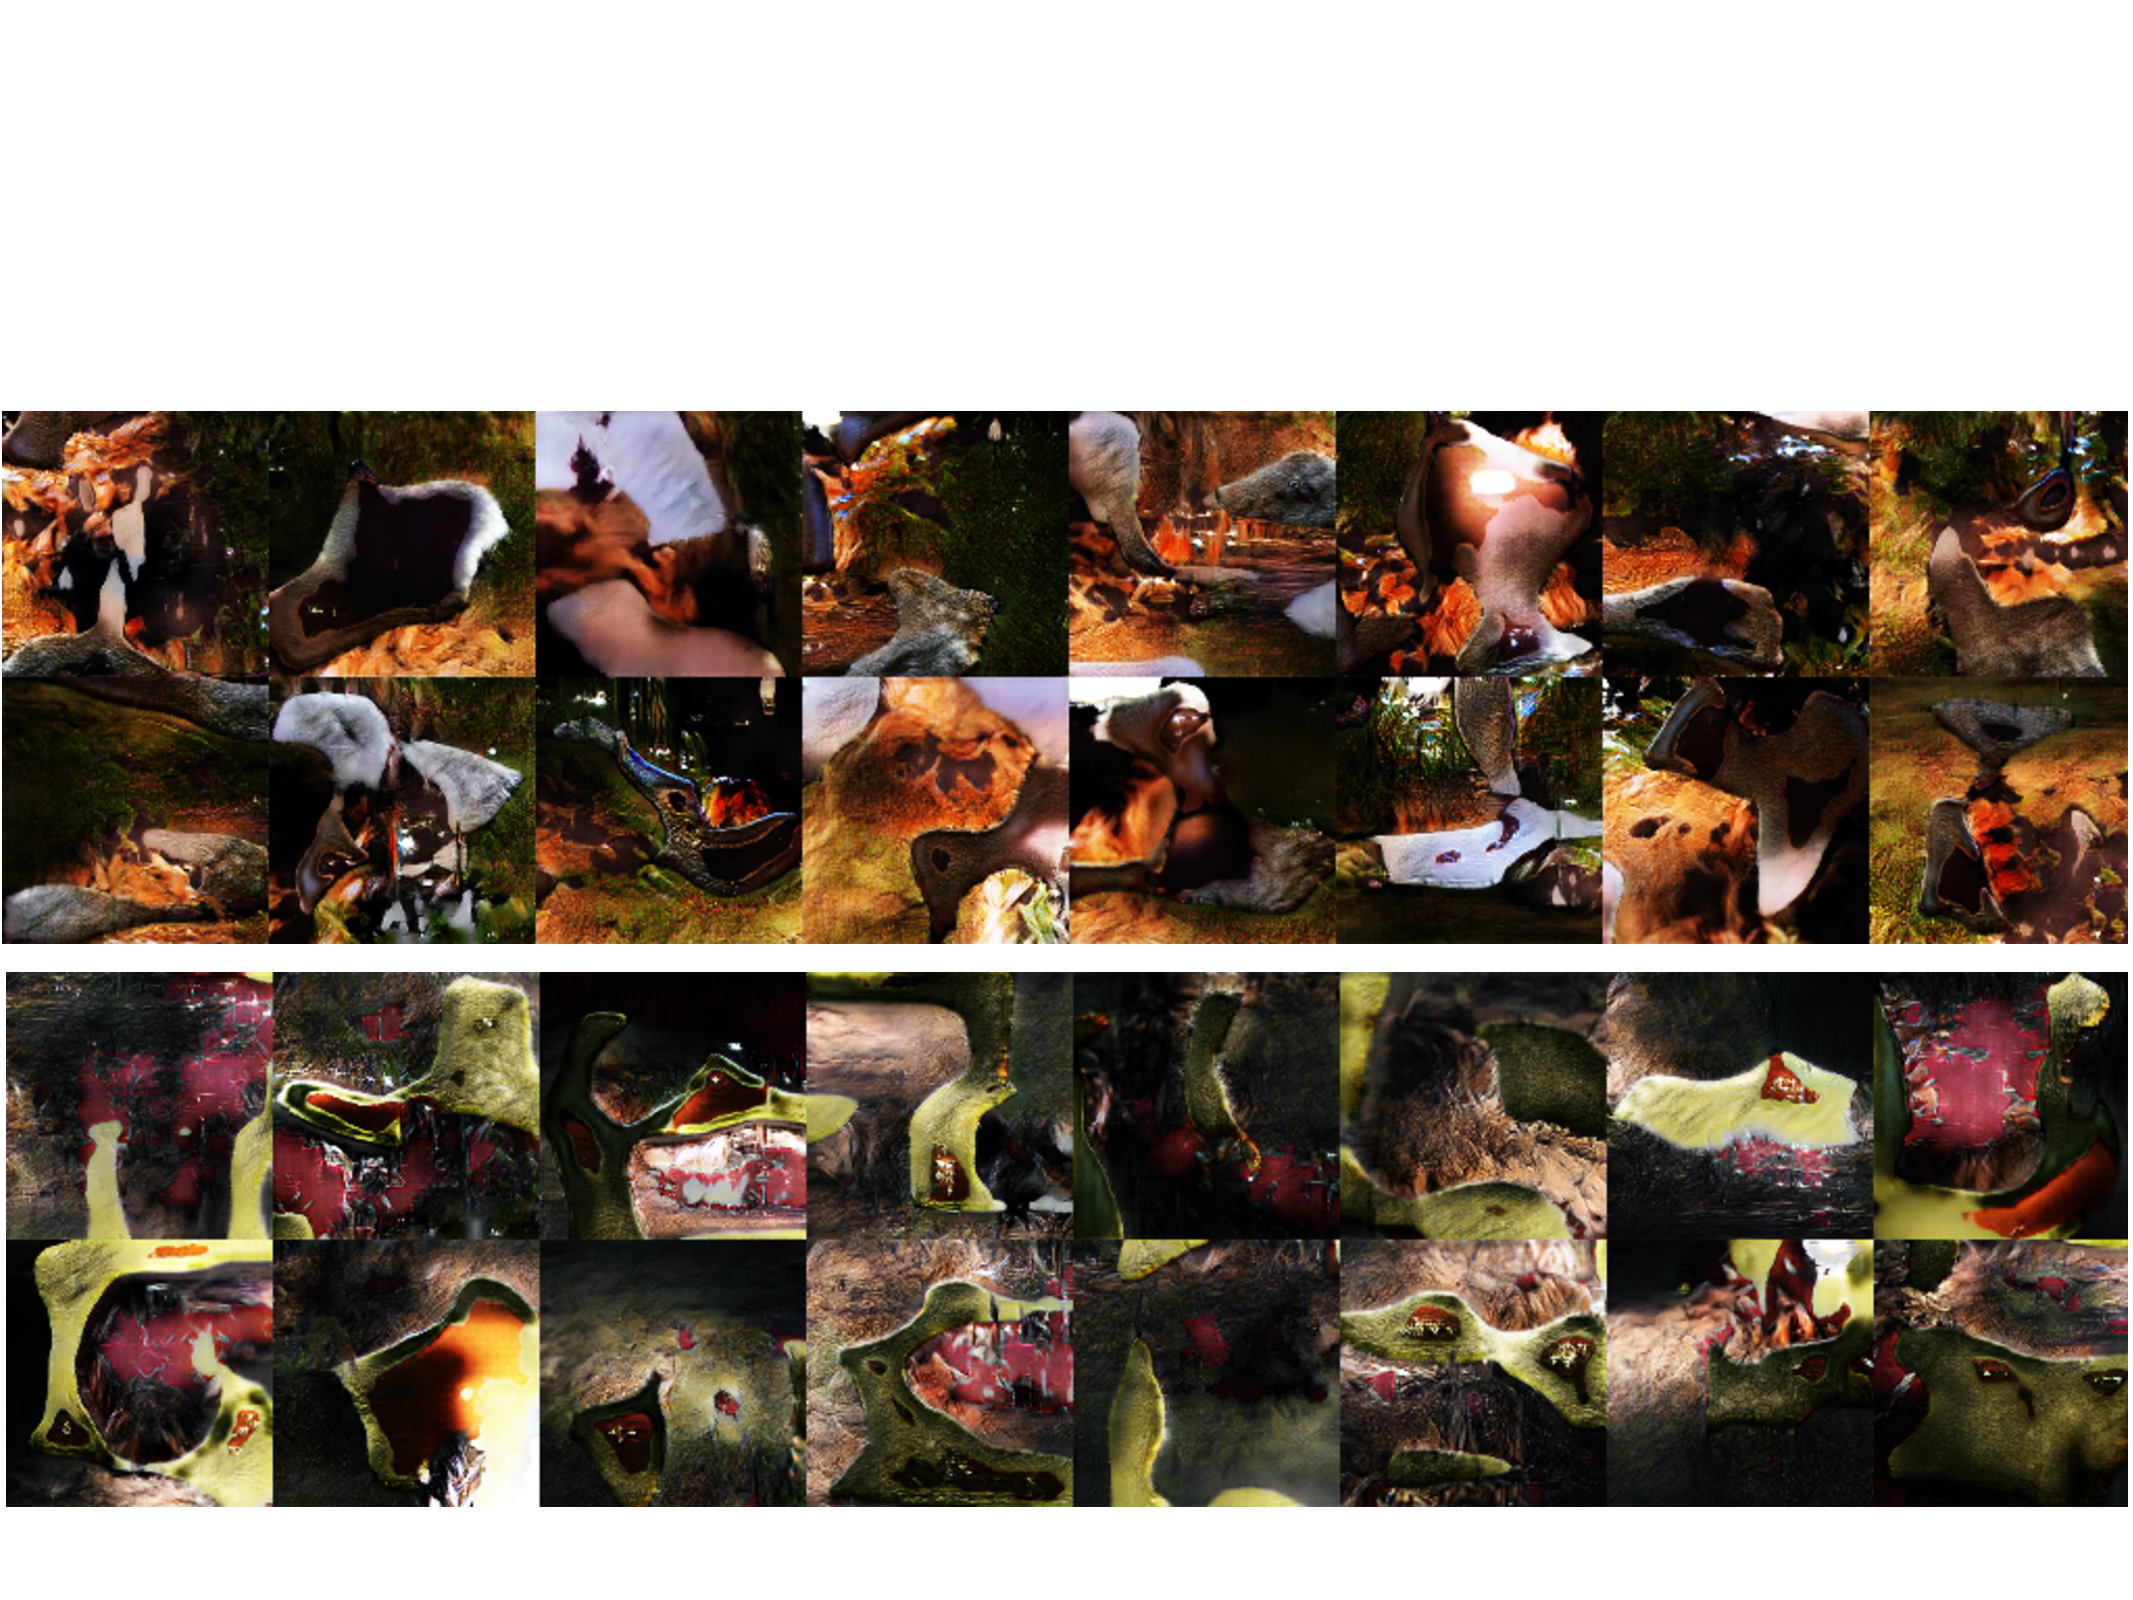
\includegraphics[width=\figwidth]{bad_batchnorm}
\caption{
Two minibatches of sixteen samples each, generated by a generator network using
batch normalization.
These minibatches illustrate a problem that occurs occasionally when using batch
normalization: fluctuations in the mean and standard deviation of feature values
in a minibatch can have a greater effect than the individual $\vz$ codes for individual
images within the minibatch.
This manifests here as one minibatch containing all orange-tinted samples and the other
containing all green-tinted samples.
The examples within a minibatch should be independent from each other, but in this
case, batch normalization has caused them to become correlated with each other.
}
\label{fig:bad_batchnorm}
\end{figure}

\citet{Salimans-et-al-arxiv2014} introduced techniques to mitigate this problem.
\newterm{Reference batch normalization} consists of running the network twice:
once on a minibatch of \newterm{reference examples} that are sampled once at the
start of training and never replaced, and once on the current minibatch of examples
to train on.
The mean and standard deviation of each feature are computed using the reference
batch. The features for both batches are then normalized using these computed statistics.
A drawback to reference batch normalization is that the model can overfit to the
reference batch. To mitigate this problem slightly, one can instead use
\newterm{virutal batch normalization}, in which the normalization statistics for each
example are computed using the union of that example and the reference batch.
Both reference batch normalization and virtual batch normalization have the property
that all examples in the training minibatch are processed independently from each other,
and all samples produced by the generator (except those defining the reference batch)
are i.i.d.

\subsection{Can one balance $G$ and $D$?}

Many people have an intuition that it is necessary to somehow balance the two players
to prevent one from overpowering the other.
If such balance is desirable and feasible, it has not yet been demonstrated in any
compelling fashion.

The author's present belief is that GANs work by estimating the ratio of the data density
and model density. This ratio is estimated correctly only when the discriminator is
optimal, so it is fine for the discriminator to overpower the generator.

Sometimes the gradient for the generator can vanish when the discriminator becomes
too accurate.
The right way to solve this problem is not to limit the power of the discriminator,
but to use a parameterization of the game where the gradient does not vanish
(\secref{sec:heuristic}).

Sometimes the gradient for the generator can become very large if the discriminator
becomes too confident. Rather than making the discriminator less accurate, a better
way to resolve this problem is to use one-sided label smoothing (\secref{sec:label_smooth}).

The idea that the discriminator should always be optimal in order to best estimate
the ratio would suggest training the discriminator for $k > 1$ steps every time
the generator is trained for one step. In practice, this does not usually result in a
clear improvement.

One can also try to balance the generator and discriminator by choosing the model
size.
In practice, the discriminator is usually deeper and sometimes has more filters
per layer than the discriminator.
This may be because it is important for the discriminator to be able to correctly
estimate the ratio between the data density and generator density, but it may
also be an artifact of the mode collapse problem---since the generator tends not
to use its full capacity with current training methods, practitioners presumably
do not see much of a benefit from increasing the generator capacity.
If the mode collapse problem can be overcome, generator sizes will presumably
increase. It is not clear whether discriminator sizes will increase proportionally.


